\documentclass{beamer}
\usepackage[utf8]{inputenc}
\usepackage[ngerman]{babel}
\usepackage{graphicx}
\usepackage[export]{adjustbox}
\usepackage{listings}
\usetheme{AnnArbor}
\usecolortheme{beaver}
\setbeamertemplate{footline}%{infolines theme}
{
\leavevmode%
\hbox{%
\begin{beamercolorbox}[wd=.333333\paperwidth,ht=2.25ex,dp=1ex,center]{author in head/foot}%
\usebeamerfont{author in head/foot}\insertshortauthor%~~(\insertshortinstitute)
\end{beamercolorbox}%
\begin{beamercolorbox}[wd=.333333\paperwidth,ht=2.25ex,dp=1ex,center]{title in head/foot}%
\usebeamerfont{title in head/foot}\insertshorttitle
\end{beamercolorbox}%
\begin{beamercolorbox}[wd=.333333\paperwidth,ht=2.25ex,dp=1ex,right]{date in head/foot}%
\usebeamerfont{date in head/foot}\insertshortdate{}\hspace*{2em}
\insertframenumber{} / \inserttotalframenumber\hspace*{2ex}
\end{beamercolorbox}}%
\vskip0pt%
}

\begin{document}
\title{Multimedia Datenformate \\
Projekttitel}
\author{Panteleimon Cheropolous, Samy Dafir, Kevin Schörgnhofer}
\institute{Fachbereich Computerwissenschaften - Universität Salzburg}
\date{30. Juni 2017}

\frame{\titlepage}

\frame{\frametitle{Inhalt}\tableofcontents}

\section{Section 1}
\frame{\frametitle{Intro}
General incentive of this assignment: \\
\vspace{0.3cm}
"`Is it possible to effectively apply \textbf{video compression} for almost identical \textbf{pictures}?"' \\
\vspace{0.3cm}
$\rightarrow$ can we achieve \textit{better} results with video compression than with image compression?\\
$\rightarrow$ which codec is best suited for our purposes?\\
$\rightarrow$ how does the change of video codec parameters affect the results?\\
$\rightarrow$ how to determine the quality of the results?\\
}

\section{Setup}
\frame{\frametitle{Dataset}
The database consists of finger vein images of different fingers of different persons\\
\begin{itemize}
 \item 6 fingers per person, with 4 pictures per finger $\rightarrow$ 24 pictures per person
 \item 60 persons at all - - - 60 korrekt ?? - - - 
 \item we worked with a subset of those
\end{itemize}
 \
- - - Platzhalter Fingervenen Bilder - - -
%\begin{figure}[H]
% \centering
% 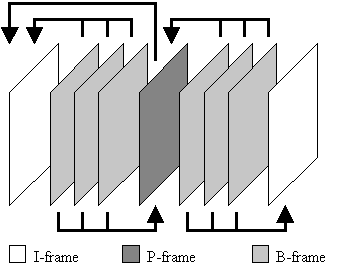
\includegraphics[width=0.5\textwidth]{graphics/ipb_frames.png}
%\end{figure}
}

\subsection{JPEG2000}
\frame{\frametitle{JPEG2000}
\begin{itemize}
 \item used as a baseline for comparison
 \item standard encoding settings, except number of layers
 \item ImageMagick with integrated OpenJPEG library
\end{itemize}
}

\subsection{I,P,B-Frames}
\frame{\frametitle{I,P,B-Frames}
% http://www.tipterminal.de/pics/ipb_frames.gif
3 different types of pictures
\begin{itemize}
 \item I-Frame: Intra-coded picture
 \item P-Frame: Predictive-coded picture
 \item B-Frame: Bidirectional predictive-coded picture
\end{itemize}
\begin{figure}[H]
 \centering
 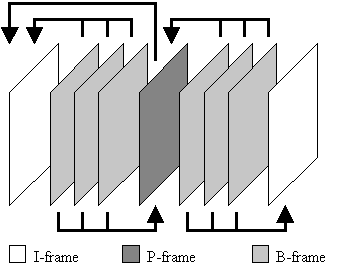
\includegraphics[width=0.5\textwidth]{graphics/ipb_frames.png}
\end{figure}
}

\subsection{Group Of Pictures}
\frame{\frametitle{Group Of Pictures}
\begin{itemize}
 \item usually defined with two numbers
 \begin{enumerate}
  \item defines distance of two I-Frames
  \item defines distance of two anchor frames (I or P)
 \end{enumerate}
 \item we used GOP to adapt the encoding to the database
 \begin{itemize}
  \item 24 pictures per person: use GOP 24 $\rightarrow$ 1 I-Frame per person
  \item 4 pictures per finger: use GOP 4 $\rightarrow$ 1 I-Frame per finger
 \end{itemize}
 \item P- and B-Frames allow higher compression $\rightarrow$ GOP affects the compression rate
\end{itemize}
}

\section{Section 2}
\subsection{Subsection 1}
\frame{\frametitle{Subsection 1}
Testtext 2.1
}

\end{document}
